\section{Realization of the Higher Order Filter}
\label{sec:implementation}

Having introduced the algorithms of building a second order recursive filter by seperating into 
particular and homogeneous functions, in this section, we move our attention on composing the higher
order recursive filter by cascading second order sec-tions.
In particular, we start at putting forward three different options of composing a second order filter
based on the algo\-rithms that we discussed. The higher order filter is then built upon
cascading different options of second order filter. 


% Having introduced the algorithms of building a second order recursive filter by seperating into 
% particular and homogeneous functions,
% in this section we systematically discuss and compare with 
% different combinations of functions of composing a second order or higher order recursive filter from implementation 
% perspective, i.e., the cost in the number of instructions. 

Three different options of composing the second order filter are given with the block diagram as follows:

1. The option 1 (benchmark): The block filtering algorithm, which only accepts a vector of samples. In particular, since the block filtering
processes with non-transposed grid of samples (to distinguish from multi-block filtering), the basic functions of block filtering
are simply named $\text{ZIC}_{\text{NT}}$ and $\text{ICC}_{\text{NT}}$, where NT stands for non-transposed grid.

% \begin{circuitikz}[node distance=1em,>=latex]%
%     \ctikzset{blocks/scale=0.8};
%     \node[coordinate] (in) [label=left:{$s(t)$}] {};
%     \node[adcshape] (adc) [right = of in, label=below:{$f_s=\frac{N}{T}$}] {};
%     \node[twoportshape] (cp) [right = of adc, t={\parbox{10em}{\centering Strip\\Cyclic\\Prefix}}] {};
%     \node[twoportshape] (sp) [right = of cp, t={S/P}] {};
%     \node[twoportshape] (fft) [right = of sp, t={FFT}] {};
%     \node[twoportshape] (eq) [right = of fft, t={Equalizer}] {};
%     \node[twoportshape] (ps) [right = of eq, t={P/S}] {};
%     \node[coordinate] (out) [right = of ps, label=right:{$s_{n}$}] {};
    
%     \draw[->] (in) -- (adc.w);
%     \draw[->] (adc.e) -- (cp.w);
%     \draw[->] (cp.e) -- (sp.w);
%     \draw[->] (sp.e) -- (fft.w);
%     \draw[->] (fft.e) -- (eq.w);
%     \draw[->] (eq.e) -- (ps.w);
%     \draw[->] (ps.e) -- (out);
%   \end{circuitikz}

\begin{equation*}
    \label{eq:option1}
    \begin{circuitikz}[node distance=1.8em,>=latex]%
        \ctikzset{blocks/scale=1.2};
        \node[coordinate] (in) [label=left:{}] {};
        \node[twoportshape] (zic) [right = of in, t={$\text{ZIC}_{\text{NT}}$}] {};
        \node[twoportshape] (icc) [right = of zic, t={$\text{ICC}_{\text{NT}}$}] {};
        \node[coordinate] (out) [right = of icc, label=right:{}] {};

        \draw[->] (in) -- (zic.w) node[near start, above]{$\bm{x}$};
        \draw[->] (zic.e) -- (icc.w) node[midway, above]{$\bm{w}$};
        \draw[->] (icc.e) -- (out) node[near end, above]{$\bm{y}$};
    \end{circuitikz}
\end{equation*}

% \begin{equation*}
%     \label{eq:option_11}
%         \begin{array}{c|c|c|c|c}
%             \cline{2-2}
%             \cline{4-4}
%             \underrightarrow{\bm{x}} & \text{NT ZIC} & \underrightarrow{\bm{w}} & \text{NT ICC} & \underrightarrow{\bm{y}} \\
%             \cline{2-2}
%             \cline{4-4}(M{\times}\bm{w})
%     \end{array}
% \end{equation*}

2. The option 2: Compared with option 1, the particular part of recursive equation is replaced by our proposed multi-block filtering,
which has the similar idea as \cite{Jaewoo_09}. The T in the box denotes the function of matrix transpose.

\begin{equation*}
    \label{eq:option2}
    \begin{circuitikz}[node distance=1.7em,>=latex]%
        \ctikzset{blocks/scale=1.2};
        \node[coordinate] (in) [label=left:{}] {};
        \node[twoportshape] (t1) [right = of in, t={T}] {};
        \node[twoportshape] (zic) [right = of t1, t={$\text{ICC}_{\text{T}}$}] {};
        \node[twoportshape] (t2) [right = of zic, t={T}] {};
        \node[twoportshape] (icc) [right = of t2, xshift=0.9cm, t={$\text{ICC}_{\text{NT}}$}] {};
        \node[coordinate] (out) [right = of icc, label=right:{}] {};

        \draw[->] (in) -- (t1.w) node[near start, above]{$\bm{X}$};
        \draw[->] (t1.e) -- (zic.w) node[midway, above]{$\bm{X}^T$};
        \draw[->] (zic.e) -- (t2.w) node[midway, above]{$\bm{W}^T$};
        \draw[->] (t2.e) -- (icc.w) node[midway, above]{$\bm{W}(M{\times}\bm{w})$};
        \draw[->] (icc.e) -- (out) node[near end, above]{$\bm{y}$};
    \end{circuitikz}
\end{equation*}


% \begin{equation*}
%     \label{eq:option_22}
%     \begin{aligned}
%         & \begin{array}{c|c|c|c|c|c|c|c|c}
%             \cline{2-2}
%             \cline{4-4}
%             \cline{6-6}
%             \cline{8-8}
%             \underrightarrow{\bm{X}} & \text{T} & \underrightarrow{\bm{X}^T} & \text{T ZIC} & \underrightarrow{\bm{W}^T} & \text{T} & \underrightarrow{\bm{W} (M \times \bm{w})} & \text{NT ICC} & \underrightarrow{\bm{y}} \\
%             \cline{2-2}
%             \cline{4-4}
%             \cline{6-6}
%             \cline{8-8}
%     \end{array}
% \end{aligned}
% \end{equation*}

3. The option 3: Our proposed multi-block filtering algorith\-m, where both of functions process with transposed matrix of samples. 

\begin{equation*}
    \label{eq:option3}
    \begin{circuitikz}[node distance=1.8em,>=latex]%
        \ctikzset{blocks/scale=1.2};
        \node[coordinate] (in) [label=left:{}] {};
        \node[twoportshape] (t1) [right = of in, t={T}] {};
        \node[twoportshape] (zic) [right = of t1, t={$\text{ICC}_{\text{T}}$}] {};
        \node[twoportshape] (icc) [right = of zic, t={$\text{ICC}_{\text{T}}$}] {};
        \node[twoportshape] (t2) [right = of icc, t={T}] {};
        \node[coordinate] (out) [right = of t2, label=right:{}] {};

        \draw[->] (in) -- (t1.w) node[near start, above]{$\bm{X}$};
        \draw[->] (t1.e) -- (zic.w) node[midway, above]{$\bm{X}^T$};
        \draw[->] (zic.e) -- (icc.w) node[midway, above]{$\bm{W}^T$};
        \draw[->] (icc.e) -- (t2.w) node[midway, above]{$\bm{Y}^T$};
        \draw[->] (t2.e) -- (out) node[near end, above]{$\bm{Y}$};
    \end{circuitikz}
\end{equation*}
% \begin{equation*}
%     \label{eq:option_33}
%     \begin{aligned}
%         & \begin{array}{c|c|c|c|c|c|c|c|c}
%             \cline{2-2}
%             \cline{4-4}
%             \cline{6-6}
%             \cline{8-8}
%             \underrightarrow{\bm{X}} & \text{T} & \underrightarrow{\bm{X}^T} & \text{T ZIC} & \underrightarrow{\bm{W}^T} & \text{T ICC} & \underrightarrow{\bm{Y}^T} & \text{T} & \underrightarrow{\bm{Y}} \\
%             \cline{2-2}
%             \cline{4-4}
%             \cline{6-6}
%             \cline{8-8}
%     \end{array}
% \end{aligned}
% \end{equation*}
% In the above block diagrams,
The notations of the data flow between functions in lowercase letters represent vector of samples,
while the uppercase letters denote matrix of samples. 
% The T in box denotes the function of matrix transpose.
In option 2, $M {\times} \bm{w}$ means $M$ number of vector ($\bm{w}$) of samples.
Since the $\bm{\text{ICC}_{\text{NT}}}$ only accepts vector of samples, the way it works is simply to passing the vectors in the matrix by order.

\begin{table}[t]
    \caption{The number of SIMD instructions (per sample) for functions and options in theory}  % title of Table
    \centering % used for centering table
    \setlength{\tabcolsep}{0.9pt}
    \begin{tabular}{c|c|c|c|c} % centered columns (4 columns)
    \hline\hline %inserts double horizontal lines
    function name & FMA & shuffle & broadcast & load \\ [0.5ex] % inserts table
    \hline % inserts single horizontal line
    $\text{ZIC}_{\text{NT}}$ & $1{+}\frac{2}{M}$ & 0 & $1{+}\frac{2}{M}$ & $1{+}\frac{5}{M}$ \\ [0.5ex]
    $\text{ICC}_{\text{NT}}$ & $\frac{2}{M}$ & 0 & $\frac{2}{M}$ & $\frac{5}{M}$ \\ [0.5ex]
    $\text{ZIC}_{\text{T}}$ & $\frac{4}{M}{-}\frac{3}{M^2}$ & $\frac{2}{M^2}$ & $\frac{4}{M^2}$ & $\frac{1}{M}{+}\frac{6}{M^2}$ \\ [0.5ex]
    $\text{ICC}_{\text{T}}$ & $\frac{4\log_2M}{M^2}{+}\frac{2}{M}$ & $\frac{2\log_2M{+}2}{M^2}$ & $\frac{2}{M}{-}\frac{2}{M^2}$ & $\frac{1}{M}{+}\frac{4\log_2M{+}8}{M^2}$ \\ [0.5ex]
    T & 0 & $\frac{\log_2M}{M}$ & 0 & $\frac{1}{M}$ \\ [0.5ex]
    Option 1 & $1{+}\frac{4}{M}$ & 0 & $1{+}\frac{4}{M}$ & $1{+}\frac{9}{M}$ \\ [0.5ex]
    Option 2 & $\frac{6}{M}{-}\frac{3}{M^2}$ & $\frac{2\log_2M}{M}{+}\frac{2}{M^2}$ & $\frac{2}{M}{+}\frac{4}{M^2}$ & $\frac{3}{M}{+}\frac{8}{M^2}$ \\ [0.5ex]
    Option 3 & $\frac{6}{M}{+}\frac{4\log_2M{-}3}{M^2}$ & $\frac{2\log_2M}{M}{+}\frac{2\log_2M+4}{M^2}$ & $\frac{2}{M}{+}\frac{2}{M^2}$ & $\frac{1}{M}{+}\frac{4\log_2M{+}14}{M^2}$ \\ [1ex]
    \hline
    \end{tabular}
    \label{table:number_of_instructions} % is used to refer this table in the text
\end{table}


The number of FMAs, shuffles, broadcast and load instru\-ctions for functions 
and options are recorded in Table \ref{table:number_of_instructions}.
Due to the different sizes of samples processed in the different functions, 
the number of instructions are transferred to instructions per sample (IPS) for fair comparison.
The broadcast operation happens at when a FMA is taken between a scalar and vector, e.g.,
in \eqref{eq:block_filtering}, $\bm{A}_{[0]}\bm{y_p}[0]$, $\bm{y_p}[0]$ should be first broadcasted to
a vector in the same length of $\bm{A}_{[0]}$ including all the elements of $\bm{y_p}[0]$, then multiply.
Furthermore, the number of store per sample for each function is identical as $1/M$, thus omitted. 


We observe 
% from Table \ref{table:number_of_instructions}
that
the option 1 is relatively efficient when the processor is restricted to only deal with shorter length of SIMD instructions.
For modern CPUs, option 2 is the cheapest at the number of FMA plus shuffle.
The feature of option 3 is its structure, i.e.,
the two matrix transposes are located at the head and tail. 
If building the higher order filter by cascading option 3,
the matrix transpose at the head of current section can be cancelled by
the other one at the tail of previous section.
Thus, the intermediate option 3 only takes the functions of ZIC and ICC.
The computing complexity of one section is reduce from $O(\log_2M/M)$ to $O(1/M)$.
Compared with the computing co-mplexities $O(\log_2M/M)$ for option 2 and 1 for option 1,
it can be seen our proposed algorithm
is more suitable for composing cascaded form of higher order recursive filter.

% the matrix transpose at the head of current section can be cancelled by the matrix transpose at the tail of previous section. 
% Thus, the intermediate second order sections of option 3
% only needs to take ZIC and ICC.
% Then, the computing complexity of one section is reduce from $O(2\log_2M/M)$ to $O(6/M)$.

\begin{figure}[t]
    \centerline{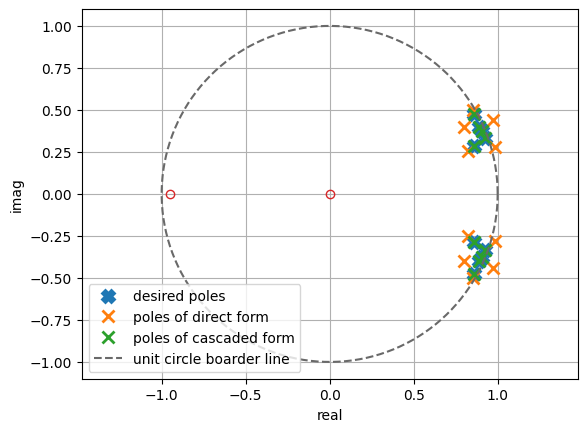
\includegraphics[width=3.3in]{poles_compare_zoom_5.png}}
    \caption{The zero-pole plot of a 10th order recursive filter in direct and cascaded form with rounding error}
    \label{fig:poles_compare_zoom}
\end{figure}

Thus, if we compare with the number of FMAs and shuffles,
then for building a $L(\geq 2)$th order recursive filter,
the smallest combination could be $L/2{-}1$ option 3 followed by one option 2.
However, there is one problem should be discussed,
i.e., the block filtering of the ICC part for option 2 inherently suffers a strong dependency
problem between vectors compared with multi-block filtering, which cannot be reflected by the number of instructions. 
Related to the parallel processor architecture that we used in this paper,
the dependency problem is going to cause the pipeline stalling.
Furthermore, since the superscalar allows 
multiple instructions to be executed simultaneously,
the clock cycles of some instruction can be overlapped by other 
instructions.
Thus, counting the number of instructions is not absolute accurate.
Due to the same reason, all the discussions of algorithms' efficiency
related to the number of instructions ignore the broadcast and load 
in this paper
because they take smaller clock cycles
than FMA and shuffle, and the cycles
will be occupied by FMAs and shuffles when
multiple instructions are executed.  
In conclusion, to compare with the performance of the algorithms, 
addtion with the number of instructions,
we should go further to see the clock cycles that
directly points to the application's latency.


% Thus, if the number of instructions is the only consideration, then
% for building a $L$th order recursive filter,
% the cheapest co-mbination could be $L/2{-}1$ option 3 followed by one option 2.
% However, there is one problem should be discussed,
% i.e., the vector filtering of the ICC part for option 2 inherently suffers a strong dependency
% problem between vectors compared with the matrix filtering, which is not reflected by the number
% of instructions. 
% If related to the parallel architecture based proc-essor 
% that we used in this paper,
% the dependency problem may cause the pipeline stalling.
% Furthermore, since the superscalar pro\-cessor allows multiple instructions to be executed 
% simultaneously,
% the clock cycle of some instruction will be overlapped 
% by other instructions, 
% thus, counting the number of instructions is not absolute accurate.
% The solution is, 
% besides the number of instructions,
% we should go further to see the clock cycles that
% directly points to the application's latency.


% Based on the above discussion, we can see that our proposed algorithm is very suitable for building cascaded form of higher order recursive filter.
% If the number of instructions is the only consideration, then for a $L$th order recursive filter,
% the cheapest combination should be $L/2{-}1$ second order filters of option 3 followed by one option 2.
% For example, the block diagram of composing a 10th order recursive filter can be given by

% \begin{equation*}
%     \label{eq:4_cascaded_option_3_1_option_2}
%     \begin{aligned}
%     & \arraycolsep=2.3pt\def\arraystretch{1.0}
%     \begin{array}{c|c|c|c|c|c|c|c|c|c|}
%         \cline{2-2}
%         \cline{4-4}
%         \cline{6-6}
%         \cline{8-8}
%         \cline{10-10}
%         \underrightarrow{\bm{X}_{(1)}} & \text{T} & \underrightarrow{\bm{X}_{(1)}^T} & \text{T ZIC} & \underrightarrow{\bm{W}_{(1)}^T} & \text{T ICC} & \underrightarrow{\bm{Y}_{(1)}^T} & \text{T ZIC} & \underrightarrow{\bm{W}_{(2)}^T} & \text{T ICC} \\
%         \cline{2-2}
%         \cline{4-4}
%         \cline{6-6}
%         \cline{8-8}
%         \cline{10-10}
%     \end{array} \\
%     & \arraycolsep=2.3pt\def\arraystretch{1.0} 
%     \begin{array}{ccc|c|c|c|c|c|c}
%         \cline{4-4}
%         \cline{6-6}
%         \cline{8-8}
%         % \cline{10-10}
%         \underrightarrow{\bm{Y}_{(2)}^T} & \cdots & \underrightarrow{\bm{Y}_{(4)}^T} & \text{T ZIC} & \underrightarrow{\bm{W}_{(5)}^T} & \text{T} & \underrightarrow{\bm{W}_{(5)}(M \times \bm{w}_{(5)})} & \text{NT ICC} & \underrightarrow{\bm{Y}_{(5)}} \\
%         \cline{4-4}
%         \cline{6-6}
%         \cline{8-8}
%         % \cline{10-10}
%     \end{array} \\
% \end{aligned}
% \end{equation*}

% However, there is one last issue should be considered at the (NT) ICC part of option 2,
% i.e., compared with matrix filtering, the vector filtering suffers a strong dependency problem since 
% the computation of current vector relies on the last two samples of previous output vector that is not reflected from the number of instructions.
% Thus, the solution is, not only to measuring the efficiency of the functions or options 
% by looking at the number of instructions, but going deeper to see the clock cycles, which 
% directly points to the application's latency.

% measuring the efficiency of the options by just looking at the number of instructions,  
% we should go deeper to see the clock cycles of the functions and options, which directly points to the 
% application's latency.
% In block filtering algorithm, the computation from each vector
% relies on the last two samples of previous output vector. Thus, 
% NT ICC may suffer from a strong dependency problem, which degrades the efficiency,
% that can't be reflected from the number of instructions.
% The solution is, instead of just looking at the number of instructions,  
% we should go deeper to see the clock cycles of the functions and options, which directly points to the 
% application's latency.


























% Having introduced the solutions of a second order recursive filter, now we discuss and compare with different
% combinations of functions to build the second or higher order recursive filter from implementation perspective.
% Assume the input is a matrix of consecutive samples. Thus, for block filtering, the functions for solving particular and homogeneous
% parts should perform $M$ times.

% The option 1 only accepts non-transposed grid of samples, i.e., the block filtering method, which can be considered as the benchmark.
% The option 2 is that the particular part of recursive equation is solved by our multi-block filtering, 
% and the vector filtering works for homogeneous part, which 
% has the same idea as the multi-block filtering method in \cite{Jaewoo_09}.
% The option 3 is our proposed multi-block filtering algorithm,
% where both functions accept the transposed matrix of samples.
% From implementation perspective,
% we are not limited to count the number of FMAs and shuffles,
% but also the number of other SIMD instructions, 
% e.g., broadcast and load operations for functions and options.
% The results are recorded in Table \ref{table:number_of_instructions}.
% The number of store for each function is identical as $1/M$, thus omitted. 
 
% \begin{table}[t]
%     \caption{The number of SIMD instructions (per sample) for functions and options in theory       }  % title of Table
%     \centering % used for centering table
%     \setlength{\tabcolsep}{0.9pt}
%     \begin{tabular}{c|c|c|c|c} % centered columns (4 columns)
%     \hline\hline %inserts double horizontal lines
%     function name & FMA & shuffle & broadcast & load \\ [0.5ex] % inserts table
%     \hline % inserts single horizontal line
%     NT ZIC & $1{+}\frac{2}{M}$ & 0 & $1{+}\frac{2}{M}$ & $1{+}\frac{5}{M}$ \\ [0.5ex]
%     NT ICC & $\frac{2}{M}$ & 0 & $\frac{2}{M}$ & $\frac{5}{M}$ \\ [0.5ex]
%     T ZIC & $\frac{4}{M}{-}\frac{3}{M^2}$ & $\frac{2}{M^2}$ & $\frac{4}{M^2}$ & $\frac{1}{M}{+}\frac{6}{M^2}$ \\ [0.5ex]
%     T ICC & $\frac{4\log_2M}{M^2}{+}\frac{2}{M}$ & $\frac{2\log_2M{+}2}{M^2}$ & $\frac{2}{M}{-}\frac{2}{M^2}$ & $\frac{1}{M}{+}\frac{4\log_2M{+}8}{M^2}$ \\ [0.5ex]
%     Transpose & 0 & $\frac{\log_2M}{M}$ & 0 & $\frac{1}{M}$ \\ [0.5ex]
%     Option 1 & $1{+}\frac{4}{M}$ & 0 & $1{+}\frac{4}{M}$ & $1{+}\frac{9}{M}$ \\ [0.5ex]
%     Option 2 & $\frac{6}{M}{-}\frac{3}{M^2}$ & $\frac{2\log_2M}{M}{+}\frac{2}{M^2}$ & $\frac{2}{M}{+}\frac{4}{M^2}$ & $\frac{1}{M}{+}\frac{10}{M^2}$ \\ [0.5ex]
%     Option 3 & $\frac{6}{M}{+}\frac{4\log_2M{-}3}{M^2}$ & $\frac{2\log_2M}{M}{+}\frac{2\log_2M+4}{M^2}$ & $\frac{2}{M}{+}\frac{2}{M^2}$ & $\frac{1}{M}{+}\frac{4\log_2M{+}14}{M^2}$ \\ [1ex]
%     \hline
%     \end{tabular}
%     \label{table:number_of_instructions} % is used to refer this table in the text
% \end{table}

% From Table \ref{table:number_of_instructions}, we basically see that the algorithms are scaled linearly by the length of SIMD instructions,
% i.e., the number of instructions per sample is inversely propotional to $M$ or $M^2$. 
% NT ZIC (or NT ICC) simply denotes the function of block filtering method for solving the particular (or homogeneous) part of recursive equation,
% where NT stands for non-transposed grid of samples (the samples are processed consecutively in vector) to distinguish from transposed grid of samples
% in multi-block filtering. 
% Assume the algorithms are implemented on software.
% Note, the load and broadcast operations are normally cheap, moreover,
% are known to the compiler at the compile time. The smart compiler will interleave
% the two operations between FMAs and shuffles to reduce the clock cycles of the program.


% On the other hand, if we re-compare each function by the total number of FMAs and shuffles, we may get similar results as before since the complexity degree for basic functions don't change.

% Let's go beyond the function level to see the three options of compusing the second order filter. Option 1 is more useful when the processor is limited to deal with the SIMD instruction.
% For modern CPUs, option 2 is the cheapest at the number of FMAs and shuffles. The feature of option 3 is that the two matrix transposes
% are located at the head and tail (one for input to ZIC, one for getting correct order of samples). When a high order recursive filter is constructed by cascading second order sections,
% the matrix transpose at the head of current section 
% can be cancelled out by the matrix transpose at the tail of previous section. 
% Thus, each intermediate cascaded second order filters of option 3 only needs to take the functions of ZIC and ICC.
% Then, the computing complexity of the intermediate sections is reduce to $O(6/M)$.


% Then, the computing complexity of intermediate sections of option 3 is $O(\log_2M/M^2)$, which is smaller than the complexity $O(\log_2M/M)$
% of option 2.

% Now we can see that our proposed algorithm is very suitable for building cascaded form of high order recursive filter.
% If the number of instructions is only the consideration, then for a $L$th order recursive filter,
% the cheapest combination can be $L/2-1$ cascaded second order filters of option 3 (without intermediate matrix transpose)
% followed by 1 second order section of option 2.

% However, there is one last problem at ICC part of option 2. In block filtering algorithm, the computation from each vector
% relies on the last two samples of previous output vector. Thus, 
% NT ICC may suffer from a strong dependency problem, which degrades the efficiency,
% that can't be reflected from the number of instructions.
% The solution is, instead of just looking at the number of instructions,  
% we should go deeper to see the clock cycles of the functions and options.





% \subsection{Combination of a second (or higher) order IIR core}

% \subsubsection{The second order IIR core}

% \begin{table}[t]
%     \caption{The number of instructions for base functions in IIR filter}  % title of Table
%     \centering % used for centering table
%     \begin{tabular}{c c c c c c} % centered columns (4 columns)
%     \hline\hline %inserts double horizontal lines
%     function name & FMA & shuffle & broadcast & load & store \\ [1ex] % inserts table
%     \hline % inserts single horizontal line
%     Transposed FIR & $2M$ & 4 & 2 & $M{+}2$ & $M$ \\ [0.3ex]
%     Non-trans FIR & $2M$ & $2M$ & 2 & $M{+}2$ & $M{+}1$ \\ [0.3ex]
%     Transposed ZIC & $2M{-}3$ & 0 & 2 & $M{+}2$ & $M$ \\ [0.3ex]
%     Non-trans ZIC & $M^2$ & 0 & $M^2$ & $2M$ & $M$ \\ [0.3ex]
%     Transposed ICC & $6M$ & 4 & $4M{+}6$ & $5M{+}6$ & $M{+}4$ \\ [0.3ex]
%     Non-trans ICC & $2M$ & 0 & $2M$ & $M{+}2$ & $M$ \\ [0.3ex]
%     Matrix transpose & 0 & $M{\log_2}M$ & 0 & $M$ & $M$ \\ [1ex]
%     \hline
%     \end{tabular}
%     \label{table:number_of_instructions} % is used to refer this table in the text
% \end{table}

% In the previous section, lots of base functions of composing a second order IIR core by passing transposed or non-transposed data are introduced.
% We now count for the number of FMAs, shuffles, broadcast, load and store operations for each base function
% as shown in Table \ref{table:number_of_instructions}. Based on the number of instructions (FMAs and shuffles) for each function,
% we list three significant combinations of a second order IIR filter and compute the total number of instructions as follows: 

% 1. Core 1: all passed non-transposed data. 
% \begin{equation*}
%     \label{eq:iir_core_1_all_non}
%     % \bm{X} = \left[\begin{array}{c|c|c|c}
%     % x[0] & x[M] & \cdots & x[M^2{-}M] \\ 
%     % x[1] & x[M{+}1] & \cdots & x[M^2{-}M{+}1] \\
%     % \vdots & \vdots & \ddots & \vdots \
%     % x[M{-}1] & x[2M{-}1] &\cdots & x[M^2{-}1] \\
%     % \end{array}\right]
%         \begin{array}{c|c|c|c|c|c|c}
%             \cline{2-2}
%             \cline{4-4}
%             \cline{6-6}
%             \underrightarrow{\bm{X}} & \text{FIR} & \underrightarrow{\bm{V}} & \text{ZIC} & \underrightarrow{\bm{W}} & \text{ICC} & \underrightarrow{\bm{Y}} \\
%             \cline{2-2}
%             \cline{4-4}
%             \cline{6-6}
%     \end{array}
% \end{equation*}

% 2. Core 2: all passed transposed data.
% \begin{equation*}
%     \label{eq:iir_core_2_all_trans}
%     \begin{aligned}
%     % \bm{X} = \left[\begin{array}{c|c|c|c}
%     % x[0] & x[M] & \cdots & x[M^2{-}M] \\ 
%     % x[1] & x[M{+}1] & \cdots & x[M^2{-}M{+}1] \\
%     % \vdots & \vdots & \ddots & \vdots \\
%     % x[M{-}1] & x[2M{-}1] &\cdots & x[M^2{-}1] \\
%     % \end{array}\right]
%     & \underrightarrow{\bm{X}} \\
%         & \begin{array}{|c|c|c|c|c|c|c|c|c|c}
%             \cline{1-1}
%             \cline{3-3}
%             \cline{5-5}
%             \cline{7-7}
%             \cline{9-9}
%             \text{T} & \underrightarrow{\bm{X}^T} & \text{T FIR} & \underrightarrow{\bm{V}^T} & \text{T ZIC} & \underrightarrow{\bm{W}^T} & \text{T ICC} & \underrightarrow{\bm{Y}^T} & \text{T} & \underrightarrow{\bm{Y}} \\
%             \cline{1-1}
%             \cline{3-3}
%             \cline{5-5}
%             \cline{7-7}
%             \cline{9-9}
%     \end{array}
% \end{aligned}
% \end{equation*}

% 3. Core 3: only ICC passed non-transposed data.
% \begin{equation*}
%     \label{eq:iir_core_3_icc_non_trans}
%     \begin{aligned}
%     % \bm{X} = \left[\begin{array}{c|c|c|c}
%     % x[0] & x[M] & \cdots & x[M^2{-}M] \\ 
%     % x[1] & x[M{+}1] & \cdots & x[M^2{-}M{+}1] \\
%     % \vdots & \vdots & \ddots & \vdots \\
%     % x[M{-}1] & x[2M{-}1] &\cdots & x[M^2{-}1] \\
%     % \end{array}\right]
%     % & \underrightarrow{\bm{X}} \\
%         & \begin{array}{c|c|c|c|c|c|c|c|c|c|c}
%             \cline{2-2}
%             \cline{4-4}
%             \cline{6-6}
%             \cline{8-8}
%             \cline{10-10}
%             \underrightarrow{\bm{X}} & \text{T} & \underrightarrow{\bm{X}^T} & \text{T FIR} & \underrightarrow{\bm{V}^T} & \text{T ZIC} & \underrightarrow{\bm{W}^T} & \text{T} & \underrightarrow{\bm{W}} & \text{ICC} & \underrightarrow{\bm{Y}} \\
%             \cline{2-2}
%             \cline{4-4}
%             \cline{6-6}
%             \cline{8-8}
%             \cline{10-10}
%     \end{array}
% \end{aligned}
% \end{equation*}
% The total cost for three cores are: $M^2{+}6M$, $2M{\log_2}M{+}10M{+}5$, $2M{\log_2}M{+}6M{+}1$, respectively.
% Normally, the length of SIMD vector is short, e.g., 4 or 8. Let's assume $M=8$ to achieve the better
% parallelism. Thus, the cost for three cores are calculated as 112, 133 and 97.

% If we consider the basic situation, i.e., a single CPU and single thread are used, core 3 should be
% the most instruction-saving. The feature of core 2 is that the two matrix transpose functions exist at the tail and head.
% If we construct a higher order IIR filter by cascading multiple second order IIR cores, the two matrix transpose functions
% at the tail and head can be cancelled out. In this case, the cost for core 2 can be then reduced to $10M{+}5=85$, which is cheaper
% than core 3. The advantage of core 1 is straightforward thus avoids two matrix transpose functions.
% Furthermore, if we consider a multi-CPU and multi-thread environment, the most expensive function of core 1, i.e., non-transposed ZIC,
% can be executed by inter-block parallelism and the real number of instructions can be reduce from $M^2$ to $M$. In this case, core 1 will be the most instruction-saving.

% \subsubsection{The higher order IIR system}

% Let's discuss the higher order IIR system by cascading the proposed three second order IIR cores.
% Take fourth order IIR system as an example.
% Again, if multiple CPUs and threads are used, the cascade of core 1 will be the most efficient. 
% If not, the most instruction-saving combination is core 2 followed by core 3, i.e.,

% \begin{equation*}
%     \label{eq:iir_system_4_core2_core3}
%     \begin{aligned}
%     % \bm{X} = \left[\begin{array}{c|c|c|c}
%     % x[0] & x[M] & \cdots & x[M^2{-}M] \\ 
%     % x[1] & x[M{+}1] & \cdots & x[M^2{-}M{+}1] \\
%     % \vdots & \vdots & \ddots & \vdots \\
%     % x[M{-}1] & x[2M{-}1] &\cdots & x[M^2{-}1] \\
%     % \end{array}\right]
%     & \underrightarrow{\bm{X}_{(1)}} \\
%     & \begin{array}{|c|c|c|c|c|c|c|c}
%         \cline{1-1}
%         \cline{3-3}
%         \cline{5-5}
%         \cline{7-7}
%         % \cline{10-10}
%         \text{T} & \underrightarrow{\bm{X}_{(1)}^T} & \text{T FIR} & \underrightarrow{\bm{V}_{(1)}^T} & \text{T ZIC} & \underrightarrow{\bm{W}_{(1)}^T} & \text{T ICC} & \underrightarrow{\bm{Y}_{(1)}^T(\bm{X}_{(2)}^T)} \\
%         \cline{1-1}
%         \cline{3-3}
%         \cline{5-5}
%         \cline{7-7}
%         % \cline{10-10}
%     \end{array} \\
%         & \begin{array}{c|c|c|c|c|c|c|c|c}
%             \cline{2-2}
%             \cline{4-4}
%             \cline{6-6}
%             \cline{8-8}
%             \underrightarrow{} & \text{T FIR} & \underrightarrow{\bm{V}_{(2)}^T} & \text{T ZIC} & \underrightarrow{\bm{W}_{(2)}^T} & \text{T} & \underrightarrow{\bm{W}_{(2)}} & \text{T ICC}  & \underrightarrow{\bm{Y}_{(2)}} \\
%             \cline{2-2}
%             \cline{4-4}
%             \cline{6-6}
%             \cline{8-8}
%     \end{array}
% \end{aligned}
% \end{equation*}
% The cost for the above fourth order IIR is $2M{\log_2}M{+}16M{+}6 = 182$. Thus, we can see that, for a $L(\geq 4)$th order IIR filter, if only a single CPU and thread is used,
% the optimal combination should be $L/2{-}1$ cascaded second order core 2 followed by one core 3 at the end.

% \subsection{Base function optimization}

% \begin{table}[t]
%     \caption{The number of cycles for each SIMD instruction in VCL}  % title of Table
%     \centering % used for centering table
%     \begin{tabular}{c c c c c c} % centered columns (4 columns)
%     \hline\hline %inserts double horizontal lines
%      & FMA & shuffle & broadcast & load & store \\ [1ex] % inserts table
%     \hline % inserts single horizontal line
%     Number of cycles & 4 & 2-3 & 2-3 & 0-1 & 0-1 \\ [0.3ex]
%     Throughput & 0.5 & 1 & 0.5 & 0.25 & 0.25 \\ [1ex]
%     \hline
%     \end{tabular}
%     \label{table:number_of_cycles} % is used to refer this table in the text
% \end{table}

% We should note that the problem that we discussed so far has two assumptions: 1. The number of cycles for broadcast,
% load and store operations are ignored. This will be true if the three operations take less cycles than FMA and shuffle since
% those operations will be inserted between FMAs and executed within the duration of FMAs. 
% 2. One FMA or shuffle instruction only takes one cycle. However, this is not always true.
% The cost of every SIMD instruction depends on what platform and micro-architecture are used to be implemented. For example, 
% in this paper, we implement the SIMD instructions on software via C++ programming by the mean of vector class library (VCL).
% The computer has the Intel Skylake CPU. The number of cycles that each instruction actually takes is listed in Table \ref{table:number_of_cycles},
% where the (reciprocal) throughput means the maximum number of instructions can be executed per clock cycle, e.g., the 0.5 throughput of FMA means
% at most 2 FMAs can be executed in one clock cycle.

% Because the FMA and shuffle instructions need to take more than one cycle in VCL, different computation strategy will affect the efficiency of base functions.
% We propose below three basic methods of improving the efficiency of base functions:

% 1. Interleave dependency. When the function of transposed ZIC in \eqref{eq:ZIC_w_trans} is executed, the inherent dependency should be paid attention to.
% By unrolling the loop and exchanging the order of FMAs for SIMD vector, \eqref{eq:ZIC_w_trans} can be computed more efficiently as

% \begin{equation}
%     \label{eq:interleave_dependency}
%     \begin{aligned}
%         & \bm{W}^T[0] = \bm{V}^T[0]; \\
%         & \bm{W}^T[1] = \text{mul\_add}(\bm{V}^T[0],a_1,\bm{V}^T[1]); \\
%         & \bm{W}^T[2] = \text{mul\_add}(\bm{W}^T[0],a_2,\bm{V}^T[2]); \\
%         & \bm{W}^T[3] = \text{mul\_add}(\bm{W}^T[1],a_2,\bm{V}^T[3]); \\
%         & \bm{W}^T[2] = \text{mul\_add}(\bm{W}^T[1],a_1,\bm{W}^T[2]); \\
%         & \bm{W}^T[3] = \text{mul\_add}(\bm{W}^T[2],a_1,\bm{W}^T[3]); \\
%         & \bm{W}^T[4] = \text{mul\_add}(\bm{W}^T[2],a_2,\bm{V}^T[4]); \\
%         & \quad\quad\quad\quad\quad\quad\quad\quad\quad \vdots
%     \end{aligned}
% \end{equation}
% where mul\_add($\cdot$) is the FMA instruction for SIMD operation in VCL.
% We can see that by exchanging the order of FMAs, each FMA is interleaved by two cycles, i.e.,
% the efficiency is increased roughly by two times compared with computing in order. 

% 2. Parallelize large sum-up. The expensive part of computing transposed ICC is the big matrix multiplication in \eqref{eq:ICC_init_w_trans}.
% The computation is essentially summing up all the FMAs without dependency for each of two blocks. Thus, we can compute and sum up the FMAs in parallel, and then
% add the sub sum-up together. For example, when calculate \eqref{eq:ICC_init_w_trans} in parallel two,

% \begin{equation}
%     \label{eq:parallelized_sum_up}
%     \begin{aligned}
%         & \bm{yt} = \text{mul\_add}(\bm{T}[0],\bm{W}^T[M{-}2][0],\bm{yt}); \\
%         & \bm{ys} = \text{mul\_add}(\bm{T}[M],\bm{W}^T[M{-}1][0],\bm{ys}); \\
%         & \bm{yt} = \text{mul\_add}(\bm{T}[1],\bm{W}^T[M{-}2][1],\bm{yt}); \\
%         & \bm{ys} = \text{mul\_add}(\bm{T}[M{+}1],\bm{W}^T[M{-}1][1],\bm{ys}); \\
%         & \bm{yl} = \text{mul\_add}(\bm{T}[2M],\bm{W}^T[M{-}2][0],\bm{yl}); \\
%         & \bm{yk} = \text{mul\_add}(\bm{T}[3M],\bm{W}^T[M{-}1][0],\bm{yk}); \\
%         & \bm{yl} = \text{mul\_add}(\bm{T}[2M{+}1],\bm{W}^T[M{-}2][1],\bm{yl}); \\
%         & \bm{yk} = \text{mul\_add}(\bm{T}[3M{+}1],\bm{W}^T[M{-}1][1],\bm{yk}); \\
%         & \quad\quad\quad\quad\quad\quad\quad\quad\quad \vdots
%     \end{aligned}
% \end{equation}
% where $\bm{yt}$, $\bm{ys}$ are two SIMD temporary registers for calculating $\bm{Y}^T[M{-}2]$, and
% $\bm{yl}$, $\bm{yk}$ are registers for calculating $\bm{Y}^T[M{-}1]$. It can be seen that by computing the 
% large sum-up in parallel, we increase the number of FMAs computed simultaneously to approach the throughput of FMA.
% Note, we can also exchange the order of computing $\bm{yt}$, $\bm{ys}$ and $\bm{yl}$, $\bm{yk}$ 
% to improve the efficiency as interleaving.

% 3. Mix FIR and ZIC. When construct a high order IIR filter, as we discussed, core 2 based on transposed data will be used 
% for multiple times. Compared with transposed ICC, transposed FIR and ZIC functions are much cheaper, thus may induce a large overhead.
% On the other hand, to mix executing FIR and ZIC, the inherent dependency of ZIC can be further interleaved by the operations in FIR,

% \begin{equation}
%     \label{eq:mix_fir_zic}
%     \begin{aligned}
%         & \bm{xp2} = \text{blend}(\bm{X}^T[M{-}2],x_{-2}); \\
%         & \bm{xp1} = \text{blend}(\bm{X}^T[M{-}1],x_{-1}); \\
%         & \bm{V}^T[0] = \text{mul\_add}(\bm{xp2},b_2,\bm{X}^T[0]); \\
%         & \bm{V}^T[0] = \text{mul\_add}(\bm{xp1},b_1,\bm{V}^T[0]); \\
%         & \bm{W}^T[0] = \bm{V}^T[0]; \\
%         & \bm{V}^T[1] = \text{mul\_add}(\bm{xp1},b_2,\bm{X}^T[1]); \\
%         & \bm{V}^T[1] = \text{mul\_add}(\bm{X}^T[0],b_1,\bm{V}^T[1]); \\
%         & \bm{W}^T[1] = \text{mul\_add}(\bm{V}^T[0],a_1,\bm{V}^T[1]); \\
%         & \quad\quad\quad\quad\quad\quad\quad\quad\quad \vdots
%     \end{aligned}
% \end{equation}
% where blend is the shuffle instruction in VCL. 
